\subsection{Curvature Analysis}
Curvature analysis is another key point of the technique described in \cite{referencePaper}. \newline
However, curvature calculation was not so clear and straightforward in the paper because they introduced the \textbf{second fundamental tensor} and the computation of \textbf{Hessian of depth field} by differentiating the gradient with a \textit{Sobel filter}. \newline
The approach implemented in my project, instead, is simpler. It starts from here\footnote{\url{https://madebyevan.com/shaders/curvature/}} and considers \textbf{screen-space normals of neighbouring} fragments as well as \textbf{depth of the current fragment} to compute a curvature value.
\subsubsection{Screen Space Surface Curvature Implementation}
Surface curvature is computed in screen space, using OpenGL \textit{partial derivatives functions} of the normal \textbf{dFdx}, \textbf{dFdy} and the \textit{depth} of the current fragment. However, we cannot use \textbf{z-values} directly, but we need to \textit{linearize} them as it is specified in openGL documentation\footnote{\url{https://learnopengl.com/Advanced-OpenGL/Depth-testing}}. \newline
Because of projection properties, a non-linear depth equation is used and it is proportional to 1/z. For this reason, we have good precision when z is small, so the object is \textit{close to the camera}, and much less precision when it is far away. \newline
As a result, we need to \textbf{transform} non-linear depth values of fragments back to its linear form in order to use them in \textit{surface curvature} calculation. To achieve this, we need to \textit{revert} the process of projection, re-transforming the values to textbf{normalized device coordinates (NDC)} and applying the inverse equation, using far and near planes. \newline
Surface Curvature and Linearized Depth functions are visible in \textbf{Code \ref{code:curvature}}.
\begin{lstlisting}[language=C++, caption=Curvature and LinearizeDepth functions in fragment shader,label={code:curvature}]
	
	float LinearizeDepth(float depth) 
	{
		float z = depth * 2.0 - 1.0; // back to NDC 
		return (2.0 * near * far) / (far + near - z * (far - near));	
	}


	float curvature(vec3 N_I)
	{
		// We compute curvature exploiting partial derivatives of the Enhanced Surface Normal
		vec3 dx = dFdx(N_I);
		vec3 dy = dFdy(N_I);
		float depth = LinearizeDepth(gl_FragCoord.z);
		float curvature_value = (cross(N_I - dx, N_I + dx).y - cross(N_I - dy, N_I + dy).x) * 4.0 / depth;
		return clamp(curvature_value, -1, 1);
	}		
\end{lstlisting}
A Comparison between curvature computation using normal vector or enhanced normal vector (through sharpening) is showed in \textbf{Figure \ref{fig:curvature_comparison}} that shows two subroutines created in the project.
\begin{figure}[h]
	\centering
	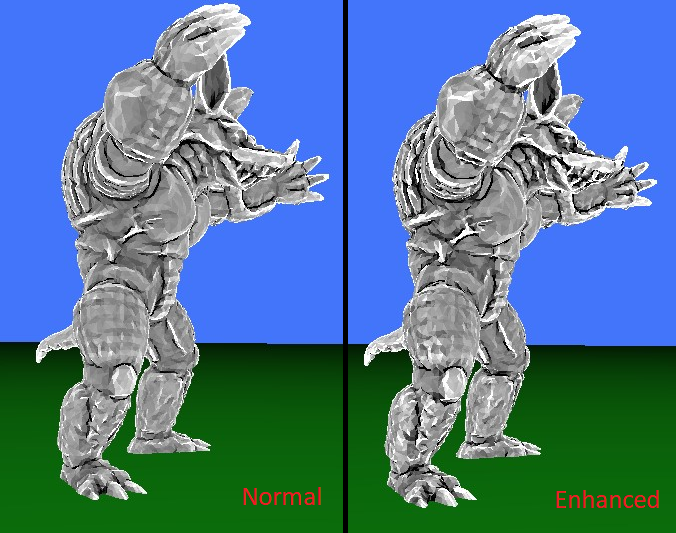
\includegraphics[width=0.8\textwidth]{Images/curvature_comparison.png}
	\caption{Comparison between curvature computation using normal vector or enhanced normal vector (through sharpening)}
	\label{fig:curvature_comparison}
\end{figure}